\xchapter{Fundamentação teórica}{}
\label{fundamentacao}

Este capítulo apresenta conceitos necessários para a compreensão do trabalho
acerca de ecossistema de software (seção \ref{sec:ecos}),
ecossistemas de software acadêmico (seção \ref{sec:ecossa}),
modelo de desenvolvimento de software acadêmico (seção \ref{sec:modelosa}),
software de análise estática (seção \ref{analise-estatica}),
sustentabilidade (seção \ref{sec:sustentabilidade}) e modelo de estágios
para ciclo de vida do software (seção \ref{sec:ciclo}).

\section{Ecossistema de software}

% ecossistema pode estar organizado em relacões de benefício mútuo

Ecossistema de software é definido, segundo \citeonline{manikas2013software},
como a interação entre diversos atores numa plataforma tecnológica comum
resultando em novas soluções de softwares ou novos serviços. Cada ator neste
sistema é motivado por um conjunto de interesses e conectam-se entre si e ao
próprio sistema numa relação simbiótica, fazendo a plataforma tecnológica
evoluir enquanto permite o envolvimento e contribuição de novos e diferentes
atores.

Nesta relação os atores são beneficiados de formas diferentes dependendo da
natureza do ecossistema, num ambiente comercial, por exemplo, os atores ganham
receita financeira diretamente (salário, prêmios, etc), enquanto num sistema
não-comercial os atores estão motivados por questões não-monetários (fama,
conhecimento, ideologia, etc).

De uma forma ou de outra, todos são beneficiados, os atores e o próprio
ecossistema, os atores recebem mais (ou melhores) benefícios com o crescimento
do ecossistema, o ecossistema oferece cada vez mais (ou melhores) benefícios
com as atividades dos seus atores, resultando numa relação de benefício
mútuo.

Este modelo geral de funcionamento do ecossistema de software pode variar a
depender do contexto em que se insere, o ecossistema de software acadêmico por
exemplo possui a particularidade de estar inserido no sistema de reputação
científica de alguma forma.

\section{Ecossistema de software acadêmico}

O ecossistema de software acadêmico possui a particularidade de estar inserido
num contexto que se relaciona com a economia de reputação científica,
especialmente com o sistema de publicação, sendo influenciado e influenciando
diretamente o impacto causado pelas suas publicações e pelo seu sistema de crédito
acadêmico.

% (5) Tools in mining software repositories \cite{chaturvedi2013tools}
% Faz uma revisão dos papers submetidos ao MSR desde 2007 até 2013 (?) e
% identifica data sets, ferramentas e técnicas utilizadas pelos autores, mais
% da metade dos papers usam ou criam ferramentas, categoriza as ferramentas em
% ferramentas novas, ferramentas tradicionais, protótipos e scripts para
% mineração de dados

\citeonline{howison2015understanding} criou um framework para pensar e refletir
sobre o processo de produção de softwares na ciência, e identificou quatro
papéis envolvidos no ecossistema de softwares acadêmicos, cientistas usuários
finais, produtores e distribuidores de software, administradores de
infraestrutura e pesquisadores preocupados com o funcionamento do ecossistema
como um todo.

\subsection{Cientistas usuários finais}

Pesquisadores de todos os domínio da ciência ocupam um papel chave no
ecossistema de software acadêmico, em seus processos de investigação e
experimentação fazem uso de artefatos de software para coletar, gerenciar,
transformar, analisar, modelar e visualizar os seus dados, sempre com o
objetivo final de publicar os seus resultados na literatura acadêmica.

Os cientistas estão preocupados com a disponibilidade, qualidade e usabilidade
destes artefatos de software e também com a capacidade de continuar úteis
podendo ser utilizados em conjunto com outros softwares. Estão interessados
também em saber o que outros cientistas usam em suas pesquisas, softwares com
alta adoção no domínio em que estão inseridos costumam manter os pesquisadores
mais livres e com maior foco em suas próprias pesquisas.

Uma alta adoção costuma ser sinal de uma boa qualidade de software, além
garantir que o grupo de pesquisa, estudantes e colaboradores consigam encontrar
mais facilmente o software e também obter ajuda entre os seus pares para
resolver questões sobre o uso do softare, simplifica também o trabalho dos
revisores pois encontrarão as mesmas facilidades no uso.

\subsection{Produtor e distribuidor de software acadêmico}

Este papel pode ser desempenhado por indivíduos ou times, softwares acadêmicos
costumam ser desenvolvidos em colaborações próximas entre cientistas da
computação e cientistas de outras áreas, usualmente sendo o cientista da
computação responsável por desenvolver algoritmos que refletem as pesquisas
destes outros pesquisadores.

Um desafio comum enfrentado pelo cientista da computação é abstrair os
problemas e implementar soluções que podem ser adotadas por outros cientistas,
especialmente em outros domínios. Alguns softwares são desenvolvidos e muitas
vezes ficam confinados em seus laboratórios ou grupos, mas eventualmente são
compartilhados e potencialmente amplamente adotados, tornando o cientista autor
do software e da pesquisa parte do ecossistema do software
\cite{howison2015understanding}.

Estes atores preocupam-se com o impacto cientifico tanto em termos de numero
quando de tipos de usuários que seu software atinge, e como seus softwares
contribuem para a ciencia que outros estão realizando.

Alguns projetos são gerenciados no estilo de código aberto, e tem atraido com
sucesso contribuições de muitos cientistas, incluindo uma calda longa de
contribuidores que tem feito pequenas mas substanciais contribuições.

\subsection{Provedor de infraestrutura}

O provedor de infraestrutura é aquele que provê um cojunto de softwares aos
cientistas usuários finais, para que dêem apoio em seus trabalhos de pesquisa.
Este conjunto de softwares podem estar disponíveis para o usuário final fazer
download eu seus computadores pessoais ou podem ser serviços de
ciberinfraestrutura de software hospedados em centros de supercomputação
usando provedores de computação em nuvem.

Do ponto de vista de ecossistema ambos os tipos de distribuição estão
interessados nas mesmas questões, quem usa ou não usa, qual versão é utilizada,
com qual frequencia atualizam, etc.

\subsection{Pesquisador}

Este último papel chamado aqui de pesquisador num sentido amplo da palavra,
refere-se à qualquer um preocupado sobre o funcionamento do próprio ecossistema
e sobre o sua contribuição para a ciência como um todo, costuma ser
desempenhado por agencias de financiamento, mas abrange qualquer cientista
preocupado com os seu trabalho individual ou do seu campo de pesquisa.

As preocupações rondam ao redor de questões sobre a operação do ecossistema como
um sistema que consome recursos (tempo, dinheiro e atenção) e afeta a conduta da
ciência, tanto no geral como em campos específicos, complementado pelo interesse
de saber como o comportamento desse sistema pode ser influenciado.

\section{Modelo de processo de softwares na ciência}

% recurso, uso e impacto

O termo ecossistema usualmente se refere a operação do sistema como um todo mas
cada ator desempenha um papel importante na estabilidade e sustentabilidade
geral do ecossistema, assim como nos ecossistemas naturais o ecossistema de
software precisa de continuas entradas (input) de energia na forma de novo
desenvolvimento ou manutenção do ecossistema \cite{dhungana2010software}.

Estes atores participam do ecossistema dentro de seus próprios interesses, mas
sempre causando um impacto de volta no sistema, os cientistas usuários finais
(direta ou indiretamente) usam softwares acadêmicos para fazer ciência,
resultando em impacto científico, este impacto científico então justifica
investimentos de novos recursos, que faz o ecossistema crescer a partir da
evolução destes softwares ou a partir da produção de novos softwares.

\begin{figure}[h]
  \center
  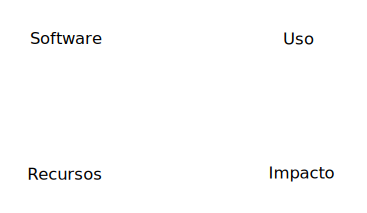
\includegraphics[scale=0.5]{imagens/process-model-scientific-software.png}
  \caption{A process model of software in science \cite{howison2015understanding}}
  \label{process-model-scientific-software}
\end{figure}

A Figura \ref{process-model-scientific-software} apresenta um diagrama deste
modelo de processo de softwares na ciência, este modelo é detalhado à seguir,
cada ator atua nos softwares, recursos, uso, impacto científico, detalhados à
seguir.

\subsection{Software}

Software acadêmico ({\it academic software}) é todo software usado para
coletar, processar ou analisar resultados de pesquisas com intenção de ser
publicados na literatura academica (seja num jornal, revista, conferência,
monografia, livro ou tese), podem ser desde protótipos escritos pelos próprios
cientistas, até mesmo produtos completos desenvolvidos profissionalmente
\cite{allen2017engineering}.

Podem ser encontrados na literatura acadêmica com outros nomes,
{\it research tool} \cite{Portillo12},
{\it research-originated software} \cite{Kon2011},
{\it research software} \cite{hettrick_2014_14809} ou
{\it scientific software} \cite{segal2008developing},
esses artefatos tem sido estudados dos mais variados pontos
de vista, desde de sua qualidade interna, até o impacto que
causam no meio científico.

No contexto de ecossistema de software acadêmico identificou-se cinco
motivações principais para a criação e contribuição ao software acadêmico:

\begin{enumerate}
  \item Ganho monetário direto (comercial software, employed software developers)
  \item Reputação acadêmica (incidental software, dirigido pela necessidade científica direta)
  \item Prática de software paralela (scientific needed enhanced by publishing 'software papers' alongside domain research)
  \item Um software de uma subárea de pesquisa (reputação direta pelo trabalho do software)
  \item Híbridos como licença-dual e 'software work' dentro de grandes colaborações (software como uma contribuição científica direta)
\end{enumerate}

\subsection{Recursos}

Os recursos investidos na produção destes softwares vem de diversas fontes,
incluem ganhos monetários diretos, recursos alocados em projetos, colaboração
entre laboratórios de pesquisa, e grande parte do ``tempo livre'' dos
pesquisadores em busca de soluções em suas pesquisas, este ``tempo livre''
perpassa por financiamentos diversos, carreira individual do cientista,
estudantes de graduação, prêmios, etc.

Independente da origem dos recursos o desenvolvimento de softwares acadêmicos
possui a particularidade de ser desenvolvido em sua grande maioria pelos
próprios cientistas uma vez que geralmente é necessário conhecimento no domínio
da pesquisa onde o software está inserido \cite{segal2008developing, hettrick_2014_14809,
momcheva2015software}.

\subsection{Uso}

% ... software é distribuido, utilizado e dá suporte à ciencia, gerando impacto ...

Estes artefatos de software são usados ativamente em diversos campos de pesquisa, como
matemática, biologia, física de partículas, astronomia, medicina e direito,
eles resolvem problemas comuns do cotidiano de pelo menos metade dos
pesquisadores de todas as áreas, desde grupos trabalhando exclusivamente com
problemas computacionais até grupos em laboratórios tradicionais ou em campo
\cite{wilson2014best}.

Os cientistas usuários finais mencionam tais softwares em suas publicações,
seja através de citação formal, informal, ou qualquer outro tipo de menção ao
software em suas pesquisas, estas citações ou menções fazem parte da economia
de reputação científica e causam impacto científico.

O impacto científico geralmente justifica o investimentos de novos recursos ao
ecossistema do software, seja para fins de planejamento, seja como
retrospectiva para avaliar os investimentos já realizados.

\subsection{Impacto científico}

% ... impacto científico justifica e potencialmente gera mais recurso ...
% \cite{katz2014transitive}

Ao longo da história, a citação formal tem sido utilizada para garantir
autenticação e autoridade, em vez de dar crédito e promover reconhecimento, na
história ocidental a citação aparece no final dos anos 1500, no início dos anos
1700 surge também no sistema legal, o ``copyright'' como reconhecendo aos
direitos autorais também surge nesse período, 1710.

A autoria das publicações tem sido realmente usado para reconhecer os autores e
contribuidores de um certo estudo, por exemplo, nos casos em que vários grupos
reivindicam crédito pelo mesmo avanço, ``backward citing'' tem sido utilizado
para verificar como as maiores comunidades de pesquisa atribuem crédito,
``forward citing'' também tem sido usada em casos onde se quer entender como
uma idéia foi usada após o seu surgimento ou publicação.

Conhecimento novo é claramente construído a partir do conhecimento passado.
Tradicionalmente, um autor cita um artigo anterior adicionando uma referência
ao autor, título, local de publicação, etc. No entanto, esse conceito não
funciona bem para produtos digitais como o software, que muitas vezes depende
de outros softwares, fragmentos de código, e algoritmos.

Este debate tem sido realizado a bastante tempo entre as diversas áreas da
bibliometria, cienciometria, altmetria e áreas similares, o fator de impacto
por exemplo proposto em 1955 apesar de continuar contribuindo para a ciência se
mostra muitas vezes utilizado da forma errada e mostra as deficiências de lidar
bem com produtos digitais gerados durante pesquisas.

\section{Sustentabilidade do ecossistema de software acadêmico}

% problemas identificados no ecossistema de software acadêmico

Um estudo sobre ecossistema de software acadêmico percebeu através dos relatos
de grande parte dos colaboradores participantes do estudo que os projetos de software
acadêmicos desenvolvidos na própria academia sofrem de {\it ``dysfunctional
chaotic churn''}, ou seja, a existência de muitos projetos, com poucos
usuários, com ciclos de vida curtos, que terminam em paralelo ao financiamento
inicial, comunidades desconectadas e paralelas, incompatibilidades entre
projetos, e tentativas aparentemente não coordenadas de ``reiniciar'' tudo
({\it re-boots}) \cite{howison2015understanding}.

Apesar de não haver evidências a respeito deste problema de forma tão abrangente,
sabe-se que parte dos problemas são realmente fato, por exemplo,
o {\it Dagstuhl Perspective Workshop}, evento organizado por um grupo de
pesquisadores sêniores de renome internacional, realizado anualmente na
universidade de Dagstuhl\footnote{\url{http://www.dagstuhl.de}} com o objetivo
refletir sobre o estado da ciência da computação explorando tópicos novos e
emergentes, em sua mais recente edição o workshop debateu sobre software
acadêmico e os problemas comuns em seu desenvolvimento, reconhecimento e
sustentabilidade \cite{allen2017engineering}.

\subsection{Desenvolvimento}

O desenvolvimento de software acadêmico ocorre em grande parte dentro da
própria academia, estudos mostram que pelo menos metade dos cientistas desenvolvem
seus próprios softwares, ao menos pacialmente, em domínios específicos este
número pode ser bem maior, na astronomia, por exemplo, estudos mostram que este
número pode chegar a 90\% \cite{hettrick_2014_14809, momcheva2015software}.

A grande participação dos cientistas no desenvolvimento destes artefatos de
software costuma ser um reflexo do tipo de conhecimento necessário ao se
desenvolver tais artefatos de software, pode ser necessário entender como o DNA
genômico se transforma em cristais de proteína, ou os meandros da dinâmica dos
fluidos, ou como resolver 20 equações diferenciais parciais simultâneas
\cite{segal2008developing}.

Desenvolvimento de software, exige algum conhecimento sobre o domínio, software
acadêmico não é diferente, mas esta grande participação dos cientistas no
desenvolvimento de software acadêmico começa a se tornar uma preocupação à
medida que a maior parte não possui treinamento algum sobre como escrever
softwares de forma eficiente, muitos não testam ou documentam os seus
softwares, faltam práticas básicas de desenvolvimento, como escrever código
legível, revisão de código, controle de versão, testes unitários, entre outros
\cite{wilson2017good}.

A qualidade dos softwares acadêmicos tem sido questionada,
a maioria também não sabe o quão confiável seu software é \cite{Merali2010Computational},
muitos estão em estado inicial de desenvolvimento \cite{marshall2013tools},
poucas foram testados fora do contexto onde foi desenvolvido \cite{Portillo12}.

Ocasionando sérios erros computacionais em conclusões centrais da literatura
acadêmica, gerando retrabalho para retratar tais erros nas mais diversas áreas
da ciência \cite{Merali2010Computational}. Dados são perdidos, análises levam
mais tempo que o necessário e os pesquisadores não conseguem a eficiência que
poderiam ter ao trabalhar com softwares acadêmicos \cite{wilson2017good}.
Causando um impacto negativo na visibilidade dos softwares acadêmicos
\cite{howison2013, katz2014transitive} e na capacidade de serem encontrados e
compartilhados.

\subsection{Reconhecimento}

% visibilidade

Apesar do crescimento no uso de software e na consequente dependência entre
cientistas de todos os campos, tornando o software acadêmico parte integral da
prática científica, apesar do apelo da comunidade científica para que o
software acadêmico seja tratado como cidadão de primeira classe, estudos tem
mostrado que muitas pesquisas não mencionam sequer o uso de software acadêmico
em suas publicações mesmo tendo feito uso de tais artefatos
\cite{momcheva2015software} \cite{howison2016software}.

Isto tem prejudicado a visibilidade do software acadêmico causando impacto
negativo em seu ecossistema, um software invisível é frequentemente excluído de
revisões por pares, uma atividade que costuma contribuir para a qualidade geral
do trabalho publicado, além disso, o
impacto negativo na visibilidade do software acadêmico faz surgir uma
série de questionamentos sobre a sua qualidade e também sobre a
capacidade de ser encontrado, compartilhado e co-desenvolvido
\cite{howison2013, katz2014transitive} \cite{howison2016software}.

Apesar de nem sempre ser possível, ou viável, ter tudo dentro de padrões
estritos, é preciso estar consciente das boas práticas ao produzir e utilizar
softwares acadêmicos, tanto para melhorar a própria abordagem quanto para
revisar outros trabalhos \cite{wilson2014best}.

Um software acadêmico em bom funcionamento devem atingir não apenas os
objetivos de entendimento e transparencia, mas também os objetivos voltados
para replicação \cite{Stodden2010}, seja logo após sua publicação, seja daqui
a 10 ou 50 anos.

\subsection{Sustentabilidade}

O desenvolvimento de software sustentável tem sido identificado como um desafio
chave no campo da ciência e da engenharia computacional, se sustentabilidade
não for levada em consideração em projetos de software, não importa qual o
domínio ou qual o propósito do software, perde-se a oportunidade de causar
mudanças positivas no planeta e na sociedade.

Apesar de sustentabilidade ser um conceito complexo e com mútiplas dimensões,
levando a debates profundos, o conceito geral é bastante simples e refe-se à
capacidade de perdurar e de continuar sendo suportado ao longo do tempo, isto
implica na qualidade de longevidade e manunetabilidade do software
\cite{venters2014software}.

Software sustentável é aquele que continua a estar disponível no futuro, em
novas plataformas, atendendo continuamente às novas necessidades do ambiente
... adequada evolução frente as condições do ambiente em constante mudança
\cite{allen2017engineering}.

Estudo mostra o decaimento das URLs ao longo do tempo, fundamenta o assunto,
mostra grafico com o caimento ao longo dos anos em publicações da
bioinformática, grafico muito bom cruzando e decaimento e tendencia com os
passar do tempo \cite{wren2017use}.

O {\it Journal of the American Statistical Association (JASA)} tem insistido na
necessiade de estarem disponíveis código e dados durante a revisão dos
manuscritos \cite{baker2016scientists}, Agências de financiamento como o {\it
US National Science Foundation} estão começando a reconhecer produtos de
pesquisa, como software, assim como fazem com as publicações, isto reconhece as
contribuições ao softwares assim como primeiro produto de pesquisa.

Isto visa especialmente garantir a longevidade dos artefatos e proporcionar que
um segundo pesquisador receba todos os benefícios do trabalho duro do primeiro
pesquisador \cite{king1995replication}, já que tanto a ciência quanto a
engenharia dependem de resultados incrementais para sua evolução. No terceiro
compromisso, relacionado ao conceito {\it desenvolvimento}, o Dagstuhl
Manifesto enfatiza a necessidade de medir a qualidade e a sustentabilidade dos
softwares científicos, tanto a priori quanto a posteriori.

\subsubsection{Manutenabilidade}

% falar de manutenabilidade como um eixo dentro de sustentabilidade técnica

A adoção e uso de softwares acadêmicos está relacionada, entre outros fatores,
também à sua qualidade, portanto é impoprtante medir e coletar sua qualidade de
alguma forma, qualidade é um vasto assunto, um dos problemas comuns enfrentado
pelos pesquisadores que desenvolvem tais softwares é a manutenabilidade
\cite{Prlic2012}.

Estudos tem mostrado que grande parte das ferramentas de software criadas na
academia estão em estado inicial de desenvolvimento \cite{marshall2013tools} e
que apenas uma pequena porcentagem são testados fora do contexto onde foi
desenvolvido \cite{Portillo12}.

%%%%%%%%%%%%%%%%%%%%%%%%%%%%%%%%%%%%%%%%%%%%%%%%%%%%%%%%%%%%%%%%%%%%%

%Cita um mapeamento feito sobre estudos que criam ferramentas para apoio a
%revisão sistemática no domínio de SE, 14 estudos foram selecionados, ao final
%apenas 8 tinham proposta de ferramentas, ao final conclui que as ferramentas
%encontradas estão em estado inicial de desenvolvimento \cite{marshall2013tools}.

%Cita um mapeamento sistemático com objetivo de encontrar ferramentas de
%comunicação e coordenação para suporte a times altamente distribuidos
%gograficamente, encontrou 132 ferramentas, para uso em projetos de software
%global. A maioria destas ferramentas foram desenvolvidas em centros de
%pesquisas, e apenas uma pequena porcentagem (18.9\%) foram testados fora do
%seu contexto onde foi desenvolvido \cite{Portillo12}.

%Computer systems research spans sub-disciplines that in-
%clude embedded and real-time systems, compilers, network-
%ing, and operating systems. Our contention is that a number
%of structural factors inhibit quality research. We highlight
%some of the factors we have encountered in our work and ob-
%served in published papers and propose solutions that could
%both increase the productivity of researchers and the quality
%of their output \cite{Vitek2011}.

%Além da aplicação, estes softwares variam também no papel que ocupam em suas
%pesquisas, alguns fazem parte dos resultados da pesquisa, como por exemplo,
%propostas de novos algoritmos ou técnicas de produção, outros são utilizados
%como parte do método de pesquisa, como coleta ou análise de dados, sendo que
%estes papeis não são excludentes.
%
%estes costumam ser citados pelos seus autores como uma das contribuições do
%estudo, seja principal ou secundária, 
%Esses softwares podem, de fato, ser um software de simulação complexo desenvolvido
%e executado em um computador de alto desempenho, mas também pode ser um
%software desenvolvido em um PC para incorporação em instrumentos; para
%manipular, analisar ou visualizar dados; ou para orquestrar fluxos de trabalho.

%e à medida
%que percebe-se que os softwares estão se tornando parte integrante dos
%processos, ferramentas e produção científicas, torna-se necessário e urgente
%discutir o seu desenvolvimento, visibilidade, qualidade e sustentabilidade.

% mostrar os beneficios da ciencia aberta, ciberinfraestrutura, etc
% * (favorecendo a ciencia e tornando a vida mais feliz para todos)

% mostrar os problemas para a ciência como um todo
% * causando problemas para o progresso de ciência, dados perdidos, etc, retrabalho
%   dificuldade de reprodução, etc...

%, não apenas técnica, mas também a
%capacidade de ser encontrado, compartilhado e co-desenvolvido, qualidades
%importantes para a evolução do próprio software, mas também extremamente útil
%para um uso eficiente dos limitados recursos da ciência \cite{howison2013,
%katz2014transitive}.

%contradizendo as boas
%práticas de qualquer projeto experimental, de ter {\it laboratory
%notebooks}\footnote{\url{https://en.wikipedia.org/wiki/Lab_notebook}}, dados
%organizados, passos documentados, e projeto estruturado para reprodutibilidade.

%softwares acadêmicos, assim
%como qualquer outro aparato experimental, são tão importantes para a ciência
%quanto são os telescópios ou tubos de ensaio \cite{wilson2014best}.

%Cientistas gastam mais tempo hoje utilizando e desenvolvendo softwares do que
%gastavam no passado.

%Software is a critical part of modern research and yet there is little support across the
%scholarly ecosystem for its acknowledgement and citation. Inspired by the activities
%of the FORCE11 working group focused on data citation, this document
%summarizes the recommendations of the FORCE11 Software Citation Working
%Group and its activities between June 2015 and April 2016. Based on a review of
%existing community practices, the goal of the working group was to produce a
%consolidated set of citation principles that may encourage broad adoption of a
%consistent policy for software citation across disciplines and venues. Our work is
%presented here as a set of software citation principles, a discussion of the motivations
%for developing the principles, reviews of existing community practice, and a
%discussion of the requirements these principles would place upon different
%stakeholders. Working examples and possible technical solutions for how these
%principles can be implemented will be discussed in a separate paper.
%\cite{smith2016software}

%Improving academic software engineering projects: A comparative study of academic and industry projects
%(compara as praticas de desenvolvimento da industria e academia e sugere melhorias, 1998!)
%https://link.springer.com/article/10.1023%2FA%3A1018925902814?LI=true

% papel pesquisador no ecossistema de soft academico
%
%Essas preocupações gerais sugerem um conjunto de questões específicas, com foco
%em padrões globais e padrões emergentes dentro do ecossistema, incluindo: Quais
%recursos foram destinados à produção de software? Quantos usuários ou
%comunidades de usuários têm projetos? Quais são os impactos científicos desse
%uso? Os números de usuários crescem? Os projetos possuem recursos e habilidades
%suficientes para gerenciar seu crescimento? Quais projetos possuem
%funcionalidades sobrepostas? Há quanto tempo os pedaços de software e projetos
%persistem? Nós desconectamos as comunidades de usuários e desenvolvedores? São
%componentes específicos, ou camadas de componentes, faltam? Que código
%geralmente é usado em conjunto; são os projetos e as pessoas que produzem esses
%componentes se comunicando adequadamente? Como podemos sustentar o software
%crítico?
%
%Aqui há uma clara tensão entre um desejo de flexibilidade e liberdade, ligado
%às expectativas de inovação científica e desejos de estruturas de autoridade e
%controle de coordenação. As questões de influência incluem: como os programas
%de financiamento e quais os requisitos em suas chamadas, resultaram em software
%amplamente utilizado e impacto científico substancial? Quais são as
%características dos campos que alcançaram maior coalescência? Quais jornais e
%conferências têm políticas exemplares? Como o trabalho de software é visto
%dentro das práticas de contratação e avaliação, como os casos de posse?
%
%\cite{howison2015understanding}

%Ao longo da história, a citação formal foi para autenticação e autoridade, em
%vez de de crédito e reconhecimento ou atribuição. A  científico citação na
%história ocidental aparece no final dos anos 1500. No início dos anos 1700, a
%citação também aparece no sistema legal como método de compreensão dos
%precedentes \cite{katz2014transitive}.

%A ideia de direitos autorais como reconhecendo aos direitos dos seus autores
%também surge nesse tempo, 1710, talvez devido a uma lenta tendência social
%societária de reconhecer a propriedade intelectual, uma idéia que parece ter se
%desenvolvido ao lado da imprensa]. Observe que a autoria de papers é realmente
%usado para notar os autores reais do artigo quanto para notar os contribuidores
%do projeto.
%Para muitos desses, o
%identificador que deve ser citado - um "nome" que se refere a um produto único
%não é claro.

%Additionally, if a cited library depends
%on another library, the contribution of this second library
%is not captured. Citation of a dataset should perhaps give
%credit to the people who gathered the data, as well as
%those who curated it, but the paper author may not know
%or be able to find these details.

%Mas independente de como seja calculado o impacto científico de uma determinada
%pesquisa o impacto causado se reverte potencialmente em mais recursos que
%poderão ser reinvestidos no próprio ecossistema onde o software está inserido.

%Science Code Manifesto \cite{barnes2013science}.
%Foco em código fonte escrito especificamente para processar dados de
%publicações, afirma que ``todo código fonte escrito especificamente para
%processar dados de uma publicação deve estar disponível para os revisores e
%leitores do paper''.

%Sustentabilidade é um conceito guarda chuva composto de múltiplas dimensões, em
%sua dimensão técnica, chamada sustentabilidade técnica, temos a preocupação com
%a longevidade da informação, dos sistemas, e infraestrutura, e sua adequada
%evolução frente as condições do ambiente em constante mudança.

%citações formais facilitam e promovem o avanço
%da ciência, mesmo diante da falta de um padrão para citar artefatos digitais
%\cite{allen2014credit}.

%Um estudo recente com 90 artigos de diversas áreas da biologia, selecionados
%aleatoriamente entre publicações usando softwares como método, mostrou que
%apenas 59 mencionavam o uso de softwares de alguma forma, os demais 31 artigos,
%apesar de usar software acadêmico, não mencionavam nada a respeito
%\cite{howison2016software}, apenas entre 31\% e 43\% das menções aos softwares
%acadêmicos envolvem citação formal.

%Não existe ainda amadurecimento suficiente sobre como citar softwares e
%outros artefatos digitais em pesquisas científicas, não temos um padrão de como fazê-lo,
%cada autor cita à sua maneira, muitas vezes ao longo do texto, outras em seções
%específicas sobre a implementação do software, nem semprem informam onde
%encontrar uma cópia do software, ou ainda nem sobre o modelo em que o software
%é distribuído, ou se é de alguma forma distribuído ao público.

%Entre os softwares acadêmicos desenvolvidos por cientistas como apoio em suas
%pesquisas, não é raro que pesquisadores deixem de disponibilizar estes artefatos,
%assim como outros desdobramentos da pesquisa, como dados e outros. Ou ainda,
%mesmo disponibilizando tais artefatos em locais de público acesso, com o tempo,
%tais locais se tornam indisponíveis inviabilizando a obtenção de tais
%artefatos.

%A comunidade tem refletido sobre os problemas relacionados ao
%desenvolvimento, promoção e sustentabilidade desses softwares, e o
%impacto que tais problemas causam no meio científico \cite{allen2017engineering}.

%, e faz
%surgir questionamentos sobre sua qualidade, não apenas técnica, mas também a
%capacidade de ser encontrado, compartilhado e co-desenvolvido, qualidades
%importantes para a evolução do próprio software, mas também extremamente úteis
%para o uso eficiente dos limitados recursos da ciência \cite{howison2013,
%katz2014transitive}.

\section{Ecossistema de software acadêmico de análise estática} \label{analise-estatica}

Ao falarmos sobre ecossistema de software acadêmico estamos nos referindo a
qualquer software, de qualquer domínio de aplicação, que tenha sido utilizado
ou produzido durante trabalhos de pesquisa com intuito de publicação na
literatura acadêmica.
%REVER - intuito de apoiar pesquisa que será eventualmente divulgada por meio da  publicação de resultados.

O ecossistema de software acadêmico de análise estática é um recorte deste
conjunto, a princípio, com as mesmas características, atores e modelo de
funcionamento, mas logicamente podendo apresentar particularidades trazidas
pela natureza do domínio de análise estática e suas ferramentas, soluções e
algoritmos.

\subsection{Análise estática}

A análise estática de código fonte é o primeiro passo para coletar informações
necessárias em diversas atividades de verificação, medição e melhoria da
qualidade de produtos de software \cite{cruz2009code, kirkov2010source}. Ela é
realizada com base no código fonte de um programa ou sistema de software, e a
partir daí descobre problemas e propriedades de sua qualidade estrutural
\cite{chess2007secure}.

Ferramentas de análise estática estão disponíveis há décadas, em especial,
para programadores. A ferramenta Lint \cite{johnson1978lint}, considerada a
primeira ferramenta de análise estática \cite{gosain2015static}, foi criada para
examinar programas escritos em linguagem C e aplicar regras de tipagem mais
estritas do que as regras dos próprios compiladores da linguagem.

Análise estática de código fonte tem como objetivo prover
informações acerca de um programa a partir do seu código fonte sem
necessidade de execução, e sem requerer qualquer outro artefato do programa
além do próprio código.

É um ramo que possui muitas das suas abordagens em comum com os estudos da
área de análise de programas ({\it program analysis}), especialmente na área de
compiladores, onde atua especialmente nas primeiras etapas do processo de compilação.

A análise estática de código fonte é considerada uma atividade meio com
objetivo de suportar uma variedade de tarefas comuns da engenharia de
software; muitas dessas tarefas são substancialmente úteis em atividades de
manutenção, incluindo \cite{binkley2007source}:

\begin{multicols}{2}
  \begin{itemize}
    \item Análise de performance
    \item Compreensão de programas
    \item Desenvolvimento baseado em modelos
    \item Detecção de clones
    \item Evolução de software
    \item Garantia de qualidade
    \item Localizaçao de falhas
    \item Manutenção de software
    \item Recuperação arquitetural
    \item Testes
  \end{itemize}
\end{multicols}

Seja em qual atividade for, a análise estática possui importância,
pois ao ser capaz de extrair informações diretamente do
código fonte de um programa, pode auxiliar a responder perguntas necessárias
para as diversas atividades de desenvolvimento e evolução de software. Essa
importância se torna ainda mais aparente diante da ``lei'' da tendência para
execução \cite{harman2010why} que indica que todos os tipos de notação tem a
tendência de se tornar executáveis.

% \subsection{Usos da análise estática de código fonte} \label{usos}

A análise de programas trata, de modo geral, da descoberta de problemas e
fatos sobre programas. Tal análise pode ser realizada sem a necessidade de executar o
programa (análise estática) ou com informações provenientes de sua execução
(análise dinâmica).

A ideia de que programas de computador podem ser utilizados para analisar
código fonte de outros programas tem uma história de mais de 40 anos.  O
programa PFORT \cite{ryder1974pfort} foi projetado para localizar potenciais
problemas na portabilidade de código Fortran; em função da diversidade de
dialetos de Fortran, uma compilação sem erros não indicava que o programa
estava correto segundo os padrões da linguagem \cite{wichmann1995industrial}.

Desde então, ferramentas de análise estática de código fonte têm surgido para
os mais diversos fins -- muitas delas a partir das pesquisas e
desenvolvimentos da área de compiladores.  O {\it parser} utilizado nessas
ferramentas têm funcionalidades análogas aos analisadores usados em
compiladores \cite{anderson2008the}.

O uso de tais ferramentas tem se tornado mais comum no ciclo de desenvolvimento de
software, sendo aplicadas em atividades distintas.
O campo de aplicação destas ferramentas é bastante variado, cobrindo diferentes
objetivos.

\subsection{Software de análise estática}

A variedade de aplicação e a constante evolução da área de análise estática, 
tanto na indústria quando na academia, resulta em  estudos teóricos e práticos, novas ferramentas, modelos e
algoritmos de análise estática. Ferramentas de análise estática têm sido
continuamente desenvolvidas e seu uso se tornado comum no ciclo de desenvolvimento de
software.

Mas apesar da rápida e constante evolução da área, ainda há carência de estudos
avaliando estas ferramentas \cite{li2010comparative}, mesmo com os avanços e com
ferramentas de sucesso, o desenvolvimento de análise estática ainda é conhecido
por ser um processo doloroso \cite{toman2017taming}.

A eficiência, confiabilidade e precisão dessas ferramentas têm sido avaliadas e
alguns estudos mostram inconsistência entre ferramentas diferentes.
Um estudo que comparou duas ferramentas de análise estática para cálculo de métricas,
revelou significantes evidências sobre a inconsistencia entre valores de métricas,
grande diferença nos valores, e discutiu quais problemas e questões levam a estas
diferenças \cite{alemerien2013experimental}.

Análise estática é a técnica mais amplamente utilizada para análise
automatizada de programas devido a sua eficiência, boa cobertura e automação.
Estudos mostram que analise estática tem grande adoção em projetos de software
livre \cite{beller2016analyzing}.
Entretanto,tecnicas de analise estatica amplamente adotadas na comunidade de software,
por exemplo, para localização de bugs e verificação de programas 
ainda sofrem um alto índice de falso-positivos \cite{gosain2015static}.

Apesar da ampla adoção de ferramentas de análise estática em estudos
acadêmicos e da crescente atenção que as técnicas de análise estática de código tem
recebido em pesquisas, nota-se ainda uma enorme distância entre a atenção dada na academia e sua adoção na indústria,
identificando um gap entre estes dois contextos \cite{ilyas2016static}.

\subsection{Software acadêmico de análise estática}

Em Ciência da Computação, particularmente em Engenharia de Software, tem-se
notado um aumento constante no número de novos softwares acadêmicos \cite{allen2017engineering},
especialmente em estudos de análise estática, 
uma área com uma longa e respeitável tradição em
pesquisas sobre a criação de novas ferramentas, métodos e algoritmos.

%Na indústria também a adoção de software de análise estática é crescente...

O software acadêmico de análise estática e o seu ecossistema, ao estar inserido
no sistema acadêmico e intimamente relacionado a economia de reputação
científica, sofre as consequências da competição que permeia este modelo, e o
seu uso invariavelmente deixa de gerar feedback positivo de volta ao seu ecossistema,
conforme Figura \ref{scientific-reputation-diagram}, onde se apresenta o
relacionamento entre a prática e a pesquisa de software acadêmico.

%está inserido no contexto similar
%a qualquer outro software acadêmico, e o seu ecossistema possui as mesmas
%características do ecossistema de software acadêmico, 

\begin{figure}[h]
  \center
  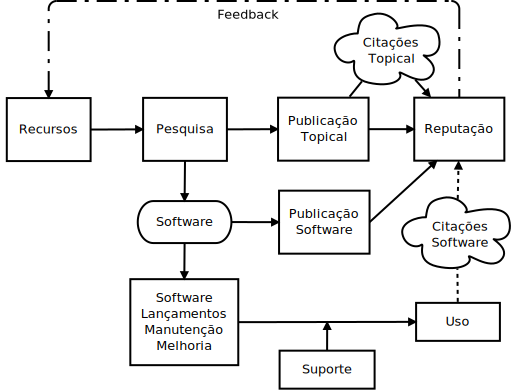
\includegraphics[scale=0.5]{imagens/scientific-reputation-diagram.png}
  \caption{Uma visão dos incentivos de reputação num contexto misto entre Ciência e práticas de software acadêmico \cite{howison2011scientific}}
  \label{scientific-reputation-diagram}
\end{figure}

%ecossistema de software acadêmico está inserido num contexto de competição

Diferentemente de outras tecnologias, software pode ser copiado e distriduído
essencialmente sem custo, abrindo portas sem precedentes em nível para
compartilhamento e inovação colaborativa \cite{howison2011scientific}, no
entanto, ao estar de alguma forma conectado ao contexto de competição da economia de
reputação científica, como no mecanismo de crédito acadêmico aos artigos e publicações,
pode ser potencialmente problemático para a colaboração e manutenção
\cite{howison2011scientific}.

%No entanto tem se percebido que o ecossistema de software acadêmico tem perdido
%oportunidade de colaboração visto que estão inseridos neste contexto ....
%competição, muitos softwares utilizados em pesquisas não são mencionados pelos
%seus autores causando impacto negativo em sua visibilidade, reconhecimento e
%consequentemente ...  \cite{howison2016software}.

Este cenário, além de desacelerar o progresso geral da Ciência gerando
retrabalho, faz surgir questionamentos sobre as conclusões dessas pesquisas,
especialmente quando grande parte dos pesquisadores não sabem o quão confiável
seus projetos de software são. Criando assim, um contexto em que muitos estudos
em Engenharia de Software sofrem de dificuldades de repetição
\cite{tang2016worthiness}, além de ocasionar problemas específicos relacionados a
manutenabilidade e sustentabilidade técnica do software acadêmico.

%Esta reflexão tem mostrado,
%por exemplo, 

%Junto com estas questões estão as questões de como
%influenciar o ecossistema, incluindo questões de pontos de inflexão que levam
%ao uso coalescente, bem como a intervenções políticas diretas incentivando o
%uso de componentes específicos.

%%%%%%%%%%%%%%%%%%%%%%%%%%%%%%%%%%%%%%%%%%%%%%%%%%%%%%%%%%%%%%

%While some of these seem relatively unproblematic, such as commercial
%production in fields with immediately valuable applications, others appear
%problematic. In particular we highlighted the potentially pernicious
%implications of the academic credit production system for collaboration and
%maintenance 

%Adicionalmente as relacões entre os atores do ecosistema como um todo
%são de mútuo interesse (mutualismo):

%O relacionamento entre os atores em um ecossistema de software, por outro lado,
%são caracterizados pela alto espectro de relacionamentos simbioticos.

%Dependendo dos atores e suas atividades, dois atores podem ter benefícios
%mútuos (mutualismo), estar em competição direta (competition/antagonism),
%estarem não afetados (neutralism) ou um não afetado enquanto o outro é
%beneficiado (amensalism) ou prejudicado (parasitism) por seu relacionamento

%em pesquisas sobre análise de código, ferramentas de analise estatica tem
%recebido significante mais atencao que outras tecnicas, tecnicas com formal e
%bem definidos processos recebem mais atencao de pesquisa e escrutinio porque
%estudos irao avaliar seu processo e elementos, entretanto, isto nao
%necessariamente significa que tecnica é melhor; The survey concluded that 1)
%the adoption of static code analysis techniques in the industry is influenced
%by the software life cycle model, while software product type and company size
%doesn’t have an influence. 2) The amount of attention a static code analysis
%technique has received in research doesn’t necessarily influence its adoption
%in industry indicating a gap between research and industry 3) company size,
%product type, and life cycle model do influence professionals perception on
%benefits/limitations.  \cite{ilyas2016static}

\section{Sustentabilidade de software acadêmico}

%\subsection{Sustentabilidade}

O desenvolvimento de software sustentável tem sido identificado como um desafio
chave no campo da ciência e da engenharia computacional, se sustentabilidade
não for levada em consideração em projetos de software, não importa qual o
domínio ou qual o propósito do software, perde-se a oportunidade de causar
mudanças positivas no planeta e na sociedade \cite{becker2014karlskrona}.

Sustentabilidade apesar de ser um conceito complexo e com mútiplas dimensões,
levando a debates profundos, possui um conceito geral bastante simples, refe-se à
capacidade de perdurar e de continuar sendo suportado ao longo do tempo, isto
implica na qualidade de longevidade e manunetabilidade do software
\cite{venters2014software}.

Software sustentável é aquele que continua a estar disponível no futuro, em
novas plataformas, atendendo continuamente às novas necessidades do ambiente
através de uma adequada evolução frente as condições em constante mudança
\cite{allen2017engineering}.

No entando, estudos mostram o decaimento de URLs ao longo do tempo, em
publicações com produção de artefatos digitais disponibilizados nestes
endereços tem uma tendência a tornarem-se indisponíveis ao longo dos anos
\cite{wren2017use}.

Isto tem motivado iniciativas de tornar estes artefatos duráveis e disponíveis,
visando especialmente garantir a longevidade dos artefatos e proporcionar que
um segundo pesquisador receba todos os benefícios do trabalho duro do primeiro
pesquisador \cite{king1995replication},
o {\it Journal of the American Statistical Association (JASA)}, por
exemplo, tem insistido na necessiade de estar disponíveis código e dados ao
menos durante a revisão dos manuscritos \cite{baker2016scientists}, agências de
financiamento, como o {\it US National Science Foundation}, estão começando a
reconhecer produtos de pesquisa, como software, assim como fazem com as
publicações, tornando o software produzido em pesquisas cidadão de primeira
classe na ciência \cite{allen2017engineering}.

Isto garante longevidade mas não implica em boa manutenabilidade, a qualidade
dos softwares acadêmicos tem sido questionada, a maioria dos cientistas autores
de software não sabe o quão confiável seu software é
\cite{Merali2010Computational}, muitos dos projetos de software acadêmico estão
em estado inicial de desenvolvimento \cite{marshall2013tools}, poucos foram
testados fora do contexto onde foram desenvolvidos \cite{Portillo12}.

\subsection{Problemas}

% problemas identificados no ecossistema de software acadêmico

O ecossistema de software acadêmico sofre de um fenômeno chamado de  
desordem caótica disfuncional ({\it ``dysfunctional chaotic
churn''}), caracterizado por:

\begin{quote}
Existência de muitos projetos, com poucos usuários, com
ciclos de vida curtos, que terminam em paralelo ao financiamento inicial,
comunidades desconectadas e paralelas, incompatibilidades entre projetos, e
tentativas aparentemente não coordenadas de ``reiniciar'' tudo ({\it re-boots})
\cite{howison2015understanding}.
\end{quote}

Este problema, apesar de ser apenas uma percepção, coincide com inúmeras
evidências a respeito de problemas com o desenvolvimento, reconhecimento e
sustentabilidade do software acadêmico \cite{allen2017engineering}.

%sabe-se que parte dos problemas são realmente fato, por exemplo,
%o {\it Dagstuhl Perspective Workshop}, evento organizado por um grupo de
%pesquisadores sêniores de renome internacional, realizado anualmente na
%universidade de Dagstuhl\footnote{\url{http://www.dagstuhl.de}} com o objetivo
%refletir sobre o estado da ciência da computação explorando tópicos novos e
%emergentes, em sua mais recente edição o workshop debateu sobre software

\subsubsection{Desenvolvimento}

O desenvolvimento de software acadêmico exige, muitas vezes, conhecimento
específico sobre o domínio do estudo sendo realizado,
por exemplo, entender como o DNA genômico
se transforma em cristais de proteína, ou estar familiarizado com os meandros
da dinâmica dos fluidos, ou saber como resolver 20 equações diferenciais
parciais simultâneas \cite{segal2008developing}.

Isto explica a grande participação dos cientistas no desenvolvimento de
software acadêmico, estudos tem mostrado que no reino unido entre todas as
áreas da ciência 56\% dos cientistas estão envolvidos no desenvolvimento de
software acadêmico \cite{hettrick2014uk}, outros estudos em grupos específicos mostram números ainda
maiores, na astronomia, por exemplo, 90\% dos cientistas desenvolvem software
acadêmico \cite{momcheva2015software}.

No entanto, a maior parte dos cientistas nunca tiveram treinamento algum sobre como escrever
softwares de forma eficiente, muitos não testam ou documentam os seus
softwares, faltam práticas básicas de desenvolvimento, como escrever código
legível, revisão de código, controle de versão, testes unitários, entre outros
\cite{wilson2017good}.

Isto tem ocasionado sérios erros computacionais em conclusões centrais da
literatura acadêmica, gerando retrabalho para retratar tais erros nas mais
diversas áreas da ciência \cite{Merali2010Computational}.
Dados são perdidos, análises levam mais tempo que o necessário e os
pesquisadores não conseguem a eficiência que poderiam ter ao trabalhar com
softwares acadêmicos \cite{wilson2017good}.
Causando um impacto negativo na visibilidade dos softwares acadêmicos e na
capacidade de serem encontrados e compartilhados \cite{howison2013,
katz2014transitive}.

\subsubsection{Reconhecimento}

% visibilidade

Apesar do crescimento no uso de software e na consequente dependência entre
cientistas de todos os campos, tornando o software acadêmico parte integral da
prática científica, apesar do apelo da comunidade científica para que o
software acadêmico seja tratado como cidadão de primeira classe, estudos tem
mostrado que muitas pesquisas não mencionam sequer o uso de software acadêmico
em suas publicações mesmo tendo feito uso de tais artefatos
\cite{momcheva2015software} \cite{howison2016software}.

Isto tem prejudicado a visibilidade do software acadêmico causando impacto
negativo em seu ecossistema, um software invisível é frequentemente excluído de
revisões por pares, uma atividade que costuma contribuir para a qualidade geral
do trabalho publicado, além disso, o
impacto negativo na visibilidade do software acadêmico faz surgir uma
série de questionamentos sobre a sua qualidade e também sobre a
capacidade de ser encontrado, compartilhado e co-desenvolvido
\cite{howison2013, katz2014transitive} \cite{howison2016software}.

Apesar de nem sempre ser possível, ou viável, ter tudo dentro de padrões
estritos, é preciso estar consciente das boas práticas ao produzir e utilizar
softwares acadêmicos, tanto para melhorar a própria abordagem quanto para
revisar outros trabalhos \cite{wilson2014best}. Um software acadêmico em bom
funcionamento devem atingir não apenas os objetivos de entendimento e
transparencia, mas também os objetivos voltados para replicação
\cite{Stodden2010}, seja logo após sua publicação, seja daqui a 10 ou 50 anos.

\subsubsection{Manutenabilidade}

% falar de manutenabilidade como um eixo dentro de sustentabilidade técnica

Manutenabilidade é uma característica de qualidade que indica o quão fácil é
realizar atividades de evolução e manutenção em software
\cite{kumar2012survey}, um aspecto importante aos pesquisadores interessados em
adaptar software acadêmico, algo muitas vezes necessário ao reproduzir
pesquisas anteriores \cite{Peng2011}.

Manutenabilidade é uma característica de qualidade externa que indica o quão
fácil é realizar atividades de evolução e manutenção em componentes de
software, ela pode ser medida através de características de qualidade interna
\cite{hashim1996software, Dagpinar2003}, uma vez que grande parte dos
engenheiros de software assumem que uma boa estrutura interna resulta em boa
qualidade externa \cite{Fenton2014}.
A estrutura interna de um software pode ser avaliada através da sua
complexidade, uma característica bastante referenciada na literatura como um
importante indicador de qualidade, estudos mostram que quanto maior a
complexidade, maior é o esforço de manutenção \cite{hashim1996software,
Darcy2005}, em especial a complexidade estrutural, uma medida definida em
termos de acoplamento e coesão \cite{Terceiro2012}.

A adoção e uso de software acadêmico está relacionado também à sua qualidade,
portanto é importante medir e coletar sua qualidade de alguma forma, qualidade
é um vasto assunto, um dos problemas comuns enfrentado pelos pesquisadores que
desenvolvem tais softwares é a manutenabilidade \cite{Prlic2012}.

Estudos tem mostrado que grande parte das ferramentas de software criadas na
academia estão em estado inicial de desenvolvimento \cite{marshall2013tools} e
que apenas uma pequena porcentagem são testados fora do contexto onde foi
desenvolvido \cite{Portillo12}.


%Iniciativas desta natureza resolvem o problema de disponibilidade destes
%artefatos mas ainda não garantem adequada evolução frente a contínua mudança
%do ambiente, apesar de sustentabilidade não implicar diretamente em qualidade,
%
%Tanto a ciência quanto a
%engenharia dependem de resultados incrementais para sua evolução. No terceiro
%compromisso, relacionado ao conceito {\it desenvolvimento}, o Dagstuhl
%Manifesto enfatiza a necessidade de medir a qualidade e a sustentabilidade dos
%softwares científicos, tanto a priori quanto a posteriori.

%Um estudo sobre ecossistema de software acadêmico percebeu através dos relatos
%de grande parte dos colaboradores participantes do estudo que os projetos de software
%acadêmicos desenvolvidos na própria academia 

\section{Ciclo de vida}

Engenheiros de software tem tradicionalmente considerado qualquer trabalho após
o primeiro lançamento de um software simplesmente como manutenção. Alguns
pesquisadores tem divido este trabalho em várias atividadesm incluindo
adaptação, prevenção, correção, entre outras, mas tem considerado manutenção
basicamente uniforme ao longo do tempo \cite{rajlich2000staged}.

No entando estudos recentes tem demonstrado que esta visão não explica muito
bem o desenvolvimento atual na maior parte dos cenários e uma das abordagens
para explicar o fenômeno tem colocado a atividade de manutenção \cite{rajlich2000staged}.

\subsection{Staged Model for Software Evolution}

O modelo {\it Staged Model for Software Evolution} \cite{rajlich2000staged}
possui cinco estágios distintos de evolução do ciclo de vida de um software,
conforme ilustrado na Figura \ref{staged-model-cycle}.  Neste modelo cada
estágio possui com atividades bastante distintas distintas, necessidades e
ferramentas variadas, e consequencias diversas no negócio.

\begin{description}
  \item [{\it Initial development.}]
    Engenheiros desenvolvem a primeira versão funcional do sistema.
  \item [{\it Evolution.}]
    Engenheiros expandem as capacidades e funcionalidades do sistema para
    atender as necessidades dos usuários.
  \item [{\it Servicing.}]
    Engenheiros fazem pequenos reparos em defeitos e mudanças funcionais
    simples.
  \item [{\it Phaseout.}]
    A empresa decide não mais oferecer serviços com o software, procurando
    gerar receita com o sistema pelo maior tempo possível.
  \item [{\it Closedown.}]
    A empresa retira o sistema do mercado e direciona os usuários para um novo
    sistema, se houver.
\end{description}

%Our work has been influenced by Franz Lehner, 2
%who provided empirical evidence that activities and
%their frequency change during a system’s life cycle.
%Manny Lehman 3 documented the inevitability of the
%evolution stage, demonstrating increases in size, com-
%plexity, and functionality during evolution.

As atividades realizadas em cada atividade variam em relação ao tipo e
frequência, na fase Evolution, por exemplo, ocorre inclusão de novas
funcionalidades, em Servicing a maior parte das alterações em código são
correções, apresentando pouca atividade com grandes mudanças mas com mudanças
frequentes enquanto durar este ciclo.

\begin{figure}[h]
  \center
  \includegraphics[scale=0.6]{imagens/staged-model-cycle.png}
  \caption{O modelo de evolução {\it staged model} consiste em cinco etapas \cite{rajlich2000staged}.}
  \label{staged-model-cycle}
\end{figure}

O retorno de uma fase para outra anterior pode representar um alto custo e alto
risco, devendo ser realizado com cautela e conhecimento deste fato.  Os
usuários devem saber em que estágio um software está antes de adquirir um
produto de software, estamos falando de produtos de software comerciais
tradicionais, para o qual este modelo de evolução foi designado e proposto.

%Transitions from one stage to the next can result
%from deliberate business decisions or by default or
%mistake. Managers must be conscious of the enormous
%business consequences of unintentional transitions and
%be aware of their symptoms so they can halt or reverse
%them while there is still time. Managers should also
%understand that attempts to return to previous stages
%or to deal with software as if it’s in a previous stage can
%be both expensive and risky.

%Customers should know what stage software is in
%and should explicitly ask for that information before
%buying it. They should avoid any software in the
%advanced servicing stage because the software is
%unlikely to evolve with the user’s needs, and close-
%down is probably near.

%• Each stage has very different technical solutions,
%processes, staff needs, and management activi-
%ties.
%• Managers who have a better understanding of
%stage transitions, their characteristics, and infor-
%mation flow across them can plan better.
%• Keeping systems within a particular stage for as
%long as possible is important.
%• Developers must design systems to allow high
%flexibility during evolution because managers can-
%not predict what new user requirements will arise.

O software acadêmico, no entando, aproxima-se muito mais de um modelo de
software livre do que de software comercial tradicional, usualmente não possuem
empresas, estão disponíveis livremente em repositórios de código fonte, e em
alguns casos são distribuídos com licenças de software livre.

\subsection{Ciclo de vida de software acadêmico}

Este modelo de evolução em estágios no entanto foi avaliado e adaptado
ao contexto de software livre \cite{capiluppi2007adapting}, e visto as
semelhanças com o software acadêmico, serve ao propósito de usar para
avaliar evolução de software acadêmico, a Figura \ref{staged-model-foss-cycle}
apresenta o modelo de evolução adaptado ao software livre, e adotado
neste estudo para software acadêmico.

\begin{figure}[h]
  \center
  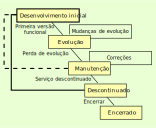
\includegraphics[scale=0.6]{imagens/staged-model-foss-cycle.png}
  \caption{O modelo de evolução {\it staged model} adaptado a software livre \cite{capiluppi2007adapting}.}
  \label{staged-model-foss-cycle}
\end{figure}

A primeira diferença observada é em relação a fase {\it Initial development},
dependendo da definição de ``fase inicial'' muitos projetos de software livre
podem nunca ter saído desta fase. Em respeito aos lançamentos,
em sistemas comerciais tradicionais eles devem ser completos, rodando e autorizado
pela empresa detentora, enquanto no mundo do software livre é comum
permitir acesso público ao código em repositórios de código fonte, seguindo
um modelo de ``versão permanente''.

A segunda diferença é relacionada a possibilidade de laços entre
as fases Evolution e Servicing. Muitos projetos de software livre
possuem fases de congelamento na adição de novas funcionalidades (freeze)
enquanto permanece numa fase de Servicing até o descongelamento, voltando
a Evolution.

A terceira diferença está na comunidade de software livre,
novos times de desenvolvimento são formados ao longo do tempo
com a saída de desenvolvedores antigos e a entrada de novos.
E projetos em fase Phaseout podem experimentar um renascimento
retornando ao período de Evolution.

Apesar das diferenças o modelo adaptado pode ser utilizado para
compreender evolução de software livre, consequentemente, também
de software acadêmico.

